\documentclass[a4paper, 12pt]{article}

%\usepackage{cmap}
\usepackage[T2A]{fontenc}
\usepackage[utf8]{inputenc}
\usepackage[english, russian]{babel}
\usepackage{graphicx}
\usepackage[top=1in, bottom=1in, left=3.2cm, right=2.6cm]{geometry}
\graphicspath{./}

\usepackage{listings}
\usepackage{color}


\begin{document}
	
\begin{titlepage}
	\fontsize{12pt}{12pt}\selectfont
	\begin{figure}[t!]
		\centering
		
\includegraphics[scale=0.8]{bmstu}
	\end{figure}
	
	\noindent\rule{15cm}{3pt}
	\newline\newline
	\noindent 
	ФАКУЛЬТЕТ 
	\underline{«Информатика и системы управления»} \newline\newline
	
	\noindent КАФЕДРА \underline{«Программное обеспечение ЭВМ и информационные технологии»}\newline\newline\newline\newline\newline\newline\newline
	
	\centering {\LARGE Отчет по лабораторной работе № 1}
	\vspace{3mm}
	
	\centering {\LARGE По курсу "Анализ Алгоритмов"
	\vspace{10mm}	
		
	\centering \bf Расстояние Левенштейна}
	\vspace{40mm}
	
	
	\begin{flushright}
		{\large	Студент:\\ Турсунов Жасурбек Рустамович \\ Группа: ИУ7-56Б
			\vspace{5mm}
			\\Преподователи: \\ Волкова Лилия Леонидовна \\ Строганов Юрий Владимирович}
	\end{flushright}
	
	\begin{center}
		\vfill
		Москва, \the\year
		~г.
	\end{center}
\end{titlepage}


\section*{Введение}

\begin{flushleft}
	 \hspace*{5mm} {\bf Расстояние Левенштейна} - минимальное количество операций вставки, удаления, замены одного символа на другой,
	необходимых для превращения одной строки в другую.
	\newline \hspace*{5mm} Расстояние Левенштейна применяется в теории информации и компьютерной лингвистике для:
	\begin{itemize}
		\item исправления ошибок в слове;
		\item сравнения текстовых файлов утилитой diff;
		\item в биоинформатике для сравнения генов, хромосом и белков;
	\end{itemize}
	\hspace*{5mm} Целью данной лабораторной работы является изучение метода динамического программирования на материале алгоритмов Левенштейна и Дамерау-Левенштейна. 
	\newline \hspace*{5mm} Задачами данной лабораторной являются: 
	\begin{enumerate}
		\item Изучение алгоритмов Левенштейна и Дамерау-Левенштейна нахождения расстояния между строками;
		\item Получение практических навыков реализации указанных алгоритмов;
		\item Сравнительный анализ линейной и рекурсивной реализаций выбранного алгоритма определения расстояний между строками по затрачиваемым ресурсам(времени);
		\item Описание и обоснование полученных результатов в отчете о выполненной лабораторной работе
    \end{enumerate}
		
\end{flushleft}
\clearpage
\newpage
\section{Аналитическая часть}
\begin{flushleft}
	\hspace*{5mm} Задача по нахождению расстояния Левенштейна заключается в поиске минимального количества операций вставки/удаления/замены для превращения одной строки в другую. При нахождении расстояния Дамерау-Левенштейна добавляется операция транспозиции(перестановки соседних символов).
	\\ {\bf Действия обозначаются так:}
	\begin{enumerate}
		\item D (англ. delete) - удалить;
		\item I (англ. insert) - вставить;
		\item R (англ. replace) - заменить;
		\item M (англ. match) - совпадение;
	\end{enumerate}
	\subsection{Алгоритм Левенштейна}
	\hspace*{5mm} Пусть $S_{1}$ и $S_{2}$ - две строки (длиной M и N соответственно) над некоторым алфавитом, тогда расстояние Левенштейна можно подсчитать по следующей рекуррентной формуле:
	\begin{figure}[h]
		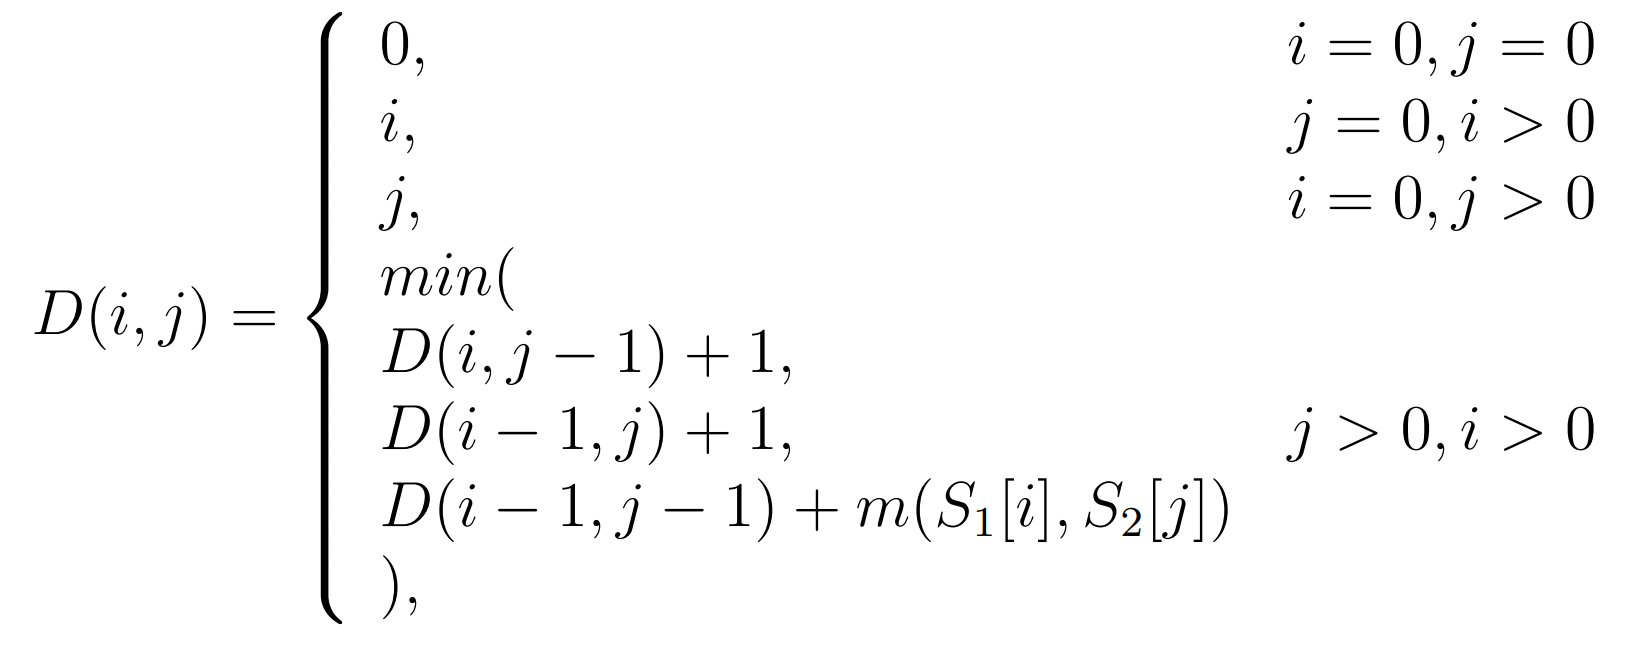
\includegraphics[scale=0.8]{lev}
	\end{figure}
	\\ где {\it m(a,b)} равна нулю, если {\it a = b} и единице в противном случае;
	\\ {\it min(a,b,c)} возвращает наименьший из аргументов.
	\newpage
	\subsection{Алгоритм Дамерау-Левенштейна}
	\hspace*{5mm} Пусть $S_{1}$ и $S_{2}$ - две строки (длиной M и N соответственно) над некоторым алфавитом, тогда расстояние Дамерау-Левенштейна можно подсчитать по следующей рекуррентной формуле:
	Расстояние Дамерау-Левенштейна вычисляются по следующей рекуррентной формуле:
	\begin{figure}[h]
		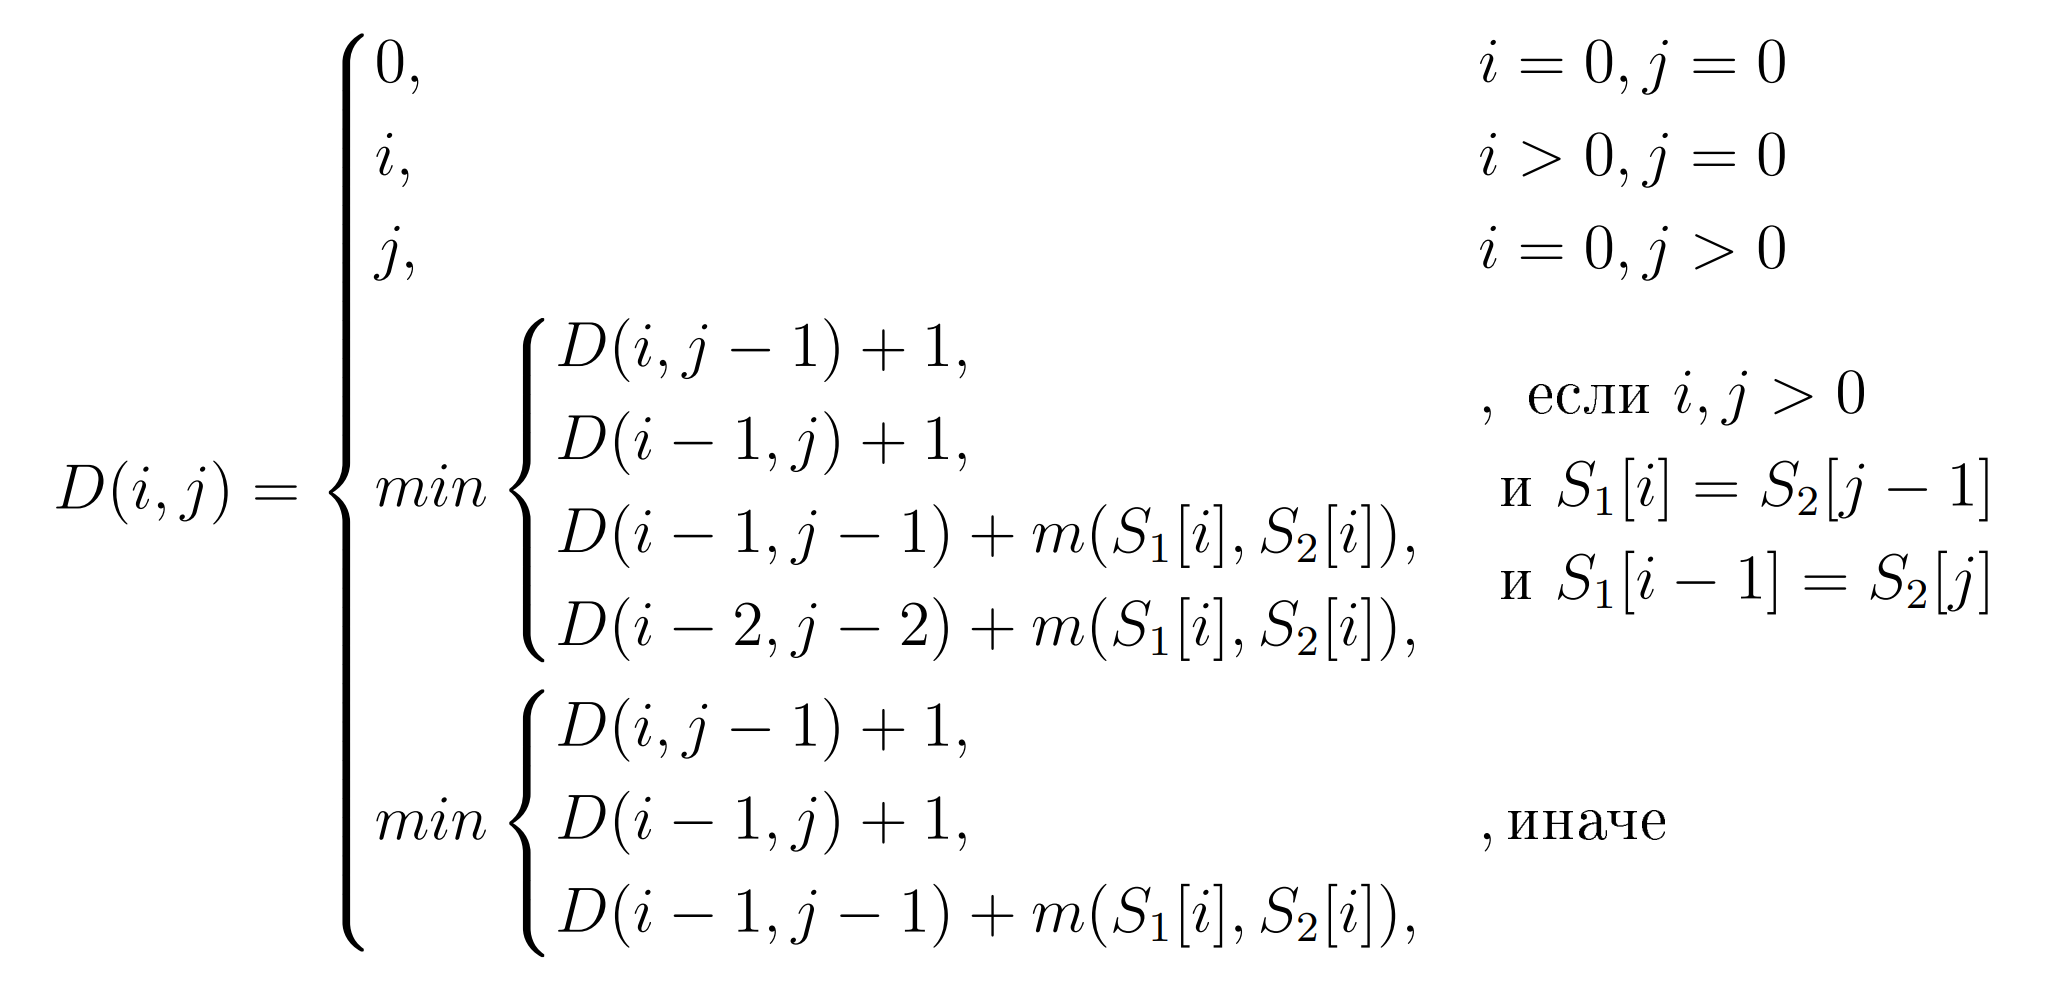
\includegraphics[scale=0.8]{damlev}
	\end{figure}
	\subsection{Вывод}
	\hspace*{5mm} Были рассмотрены поверхностно алгоритмы нахождения расстояния Левенштейна и его усовершенствованный алгоритм нахождения расстояния Дамерау-Левенштейна, принципиальная разница которого — наличие транспозиции.
\end{flushleft}

\newpage
\section{Конструкторская часть}
\begin{flushleft}
	{\bf Требования к вводу: }
	\begin{enumerate}
		\item На вход подаются две строки;
		\item Строчные и заглавные буквы считаются разными;
	\end{enumerate}

	\begin{enumerate}
		\item Две пустые строки - корректный ввод, программа не должна аварийно завершаться;
	\end{enumerate}
	\subsection{Разработка алгоритмов}
	В данном разделе будут рассмотрены схемы алгоритмов:
	\begin{itemize}
		\item Табличный алгоритм Левенштейна;
		\item Рекурсивный алгоритм Левенштейна;
		\item Табличный алгоритм Дамерау-Левенштейна;
		\item Рекурсивный алгоритм Дамерау-Левенштейна;
	\end{itemize}
	\newpage
	\begin{figure}[h]
		\centering 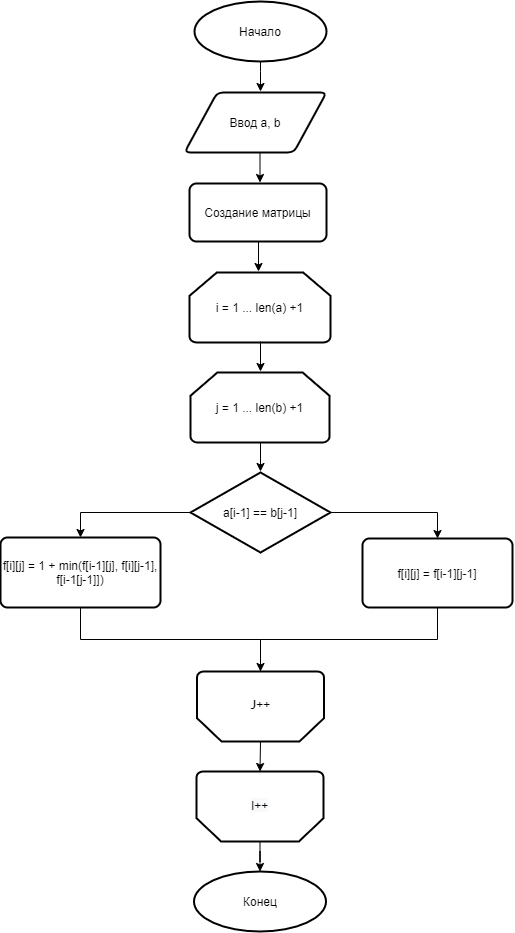
\includegraphics[scale=0.6]{diaglev}
		\centering \caption{Схема матричного алгоритма нахождения расстояния Левенштейна}
	\end{figure}
	\clearpage
	\newpage
	\begin{figure}[h]
		\centering 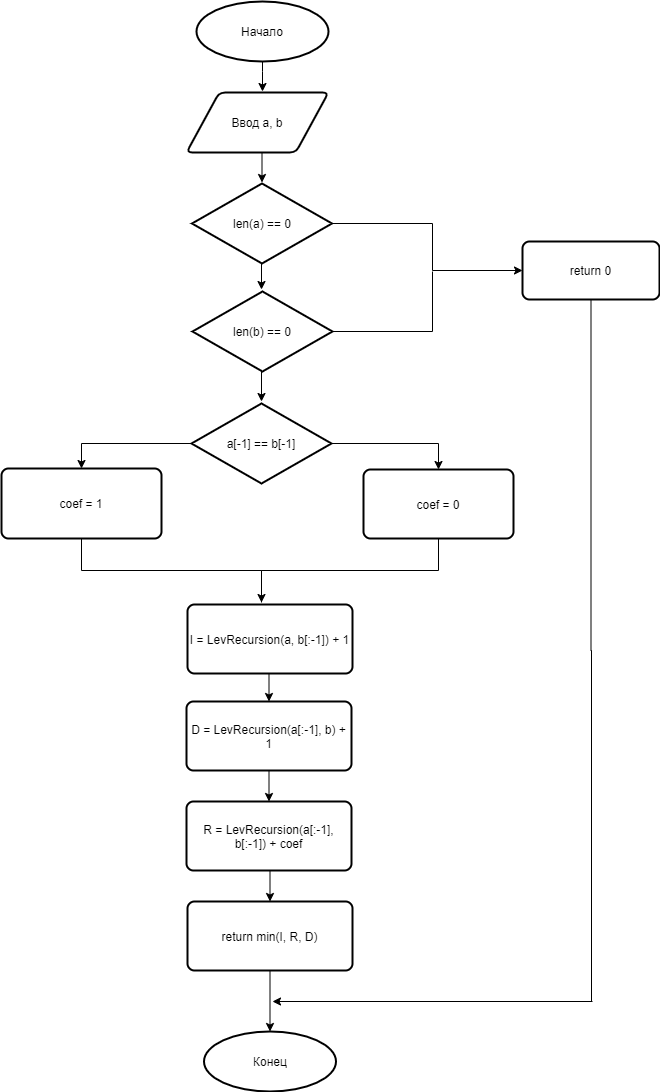
\includegraphics[scale=0.6]{levrec}
		\centering \caption{Схема рекурсивного алгоритма нахождения расстояния Левенштейна}
	\end{figure}
    \clearpage
	\newpage
	\begin{figure}[h]
		\centering 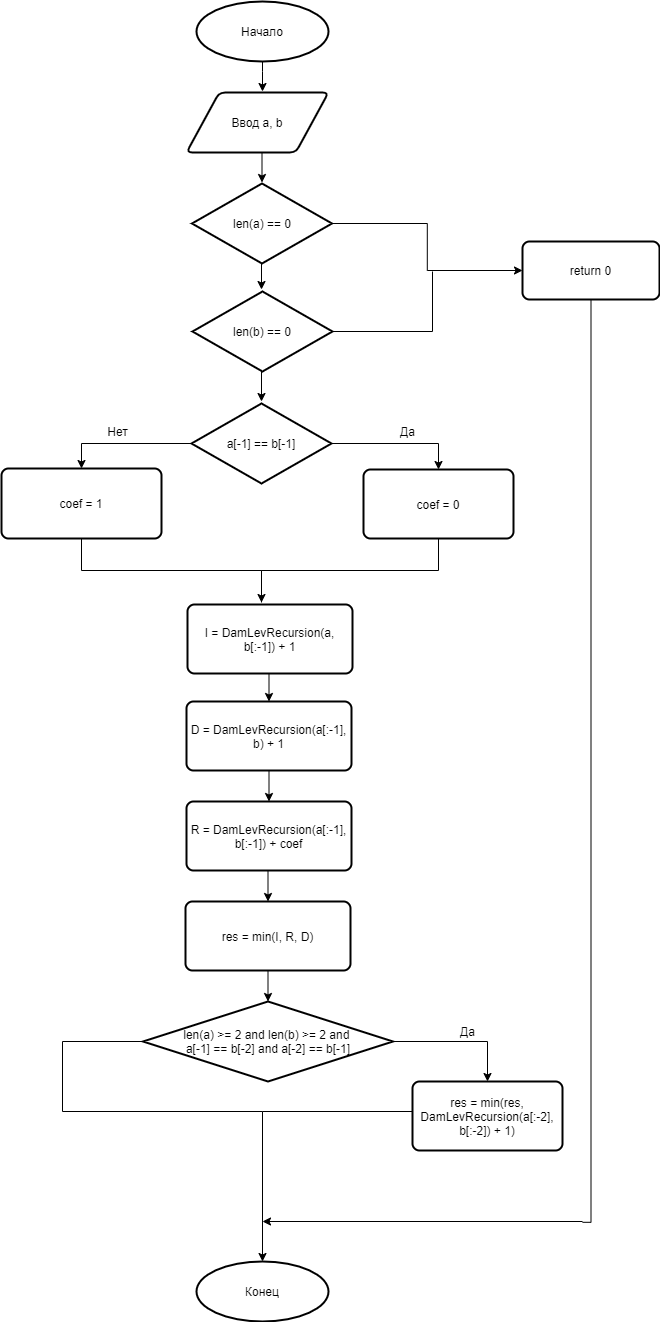
\includegraphics[scale=0.5]{damlevrec}
		\centering \caption{Схема рекурсивного алгоритма нахождения расстояния Дамерау-Левенштейна}
	\end{figure}
	\clearpage
	\newpage
	\begin{figure}[h]
		\centering 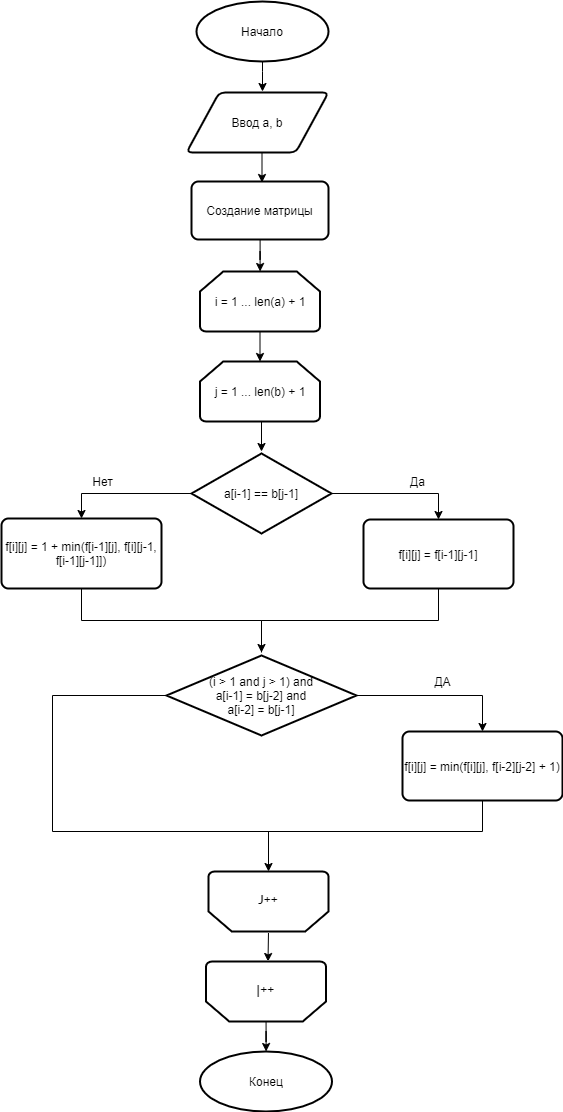
\includegraphics[scale=1.7]{damlevtable}
		\centering \caption{Схема матричного алгоритма нахождения расстояния Дамерау-Левенштейна}
	\end{figure}
    \clearpage

\end{flushleft}

\newpage
\section{Технологическая часть}
\begin{flushleft}
	\hspace*{5mm} В данном разделе будут рассмотрены требования к программному обеспечению, средства реализации и представлен листинг кода.
	\subsection{Требования к программному обеспечению}
	\hspace*{5mm} Входные данные: a - первое слово, b - второе слово.
	\\ \hspace*{5mm} Выходные данные: значение расстояние между двумя словами.
	\begin{figure}[h]
		\centering 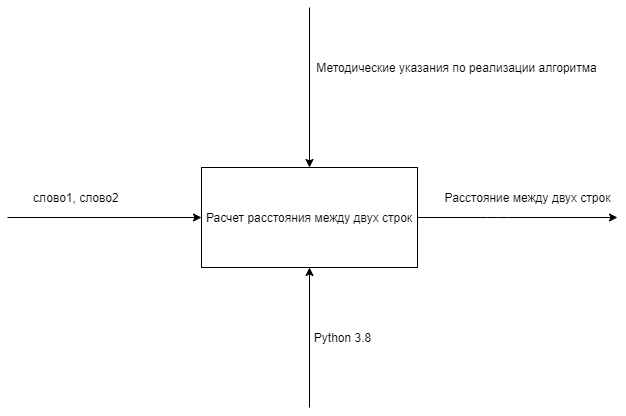
\includegraphics[scale=0.6]{диаграмма}
		\centering\caption{IDEF0-диаграмма, описывающая алгоритм нахождения расстояния Левенштейна.}
	\end{figure}
	\subsection{Средства реализации}
	\hspace*{5mm} В данной работе используется язык программирования Python, так как ЯП позволяет написать программу за кратчайшее время. Проект выполнен в среде разработки Visual Studio Code.
	\subsection{Листинг кода}
	В данном пункте представлен листинг кода, а именно:
	\begin{itemize}
		\item Расстояние Левенштейна;
		\item Рекурсивное расстояние Левенштейна;
		\item Расстояние Дамерау-Левенштейна;
		\item Рекурсивное расстояние Дамерау-Левенштейна;
	\end{itemize}
	\definecolor{codegreen}{rgb}{0,0.6,0}
	\definecolor{codegray}{rgb}{0.5,0.5,0.5}
	\definecolor{codepurple}{rgb}{0.58,0,0.82}
	\definecolor{backcolour}{rgb}{0.95,0.95,0.92}

	\lstdefinestyle{mystyle}{
		backgroundcolor=\color{backcolour},   
		commentstyle=\color{codegreen},
		keywordstyle=\color{magenta},
		numberstyle=\tiny\color{codegray},
		stringstyle=\color{codepurple},
		basicstyle=\ttfamily\footnotesize,
		breakatwhitespace=false,         
		breaklines=false,                 
		captionpos=b,                    
		keepspaces=true,                 
		numbers=left,                    
		numbersep=5pt,                  
		showspaces=false,                
		showstringspaces=false,
		showtabs=false,                  
		tabsize=4
	}

	\lstset{style=mystyle}

	\begin{lstlisting}[language=Python, caption = Расстояние Левенштейна]
	def LevTable(a, b):
		f=[[i+j if i*j==0 else 0 for j in range(len(b)+1)] 
		                         for i in range (len(a)+1)]
		for i in range(1, len(a) + 1):
			for j in range (1, len(b) + 1):
				if a[i-1] == b[j-1]:
					f[i][j] = f[i-1][j-1]
				else:
					f[i][j]=1+min(f[i-1][j], f[i][j-1], f[i-1][j-1])
		return f[len(a)][len(b)]
	\end{lstlisting}

	\begin{lstlisting}[language=Python, caption = Рекурсивное расстояние Левенштейна]
		def DamLevRecursion(a, b):
			if a ==  "" or b == "":
				return 0
			coef = 0 if (a[-1] == b[-1]) else 1
			res = min(DamLevRecursion(a, b[:-1]) + 1, 
						DamLevRecursion(a[:-1], b) + 1, 
		    			DamLevRecursion(a[:-1], b[:-1]) + coef)
			if (len(a) >= 2 and len(b) >= 2 and a[-1] == b[-2] 
											and a[-2] == b[-1]):
				res = min(res, DamLevRecursion(a[:-2], b[:-2]) + 1)
			return res 
	\end{lstlisting}

	\begin{lstlisting}[language=Python, caption = Расстояние Дамерау-Левенштейна]
		def DamLevTable(a, b):
			f = [[i+j if i*j == 0 else 0 for j in range(len(b) + 1)] 
										 for i in range (len(a) + 1)]
			for i in range(1, len(a) + 1):
				for j in range(1, len(b) + 1):
					if a[i-1] == b[j-1]:
						f[i][j] = f[i-1][j-1]
					else:
						f[i][j]=1+min(f[i-1][j],f[i][j-1],f[i-1][j-1])
					if (i > 1 and j > 1) and a[i-1] == b[j-2] 
										 and a[i-2] == b[j-1]:
						f[i][j] = min(f[i][j], f[i-2][j-2] + 1)
			return f[len(a)][len(b)]
	\end{lstlisting}
	\begin{lstlisting}[language=Python, caption = Рекурсивное расстояние Дамерау-Левенштейна]
		def DamLevRecursion(a, b):
			if a ==  "" or b == "":
				return 0
			coef = 0 if (a[-1] == b[-1]) else 1
			res = min(DamLevRecursion(a, b[:-1]) + 1,
					  DamLevRecursion(a[:-1], b) + 1,
		              DamLevRecursion(a[:-1], b[:-1]) + coef)
			if (len(a) >= 2 and len(b) >= 2 and a[-1] == b[-2] 
											and a[-2] == b[-1]):
				res = min(res, DamLevRecursion(a[:-2], b[:-2]) + 1)
			return res 
	\end{lstlisting}
	\subsection{Результаты тестирования}
	\hspace*{5mm} В данном разделе будут показаны результаты тестирования.
	\begin{figure}[h]
		\centering 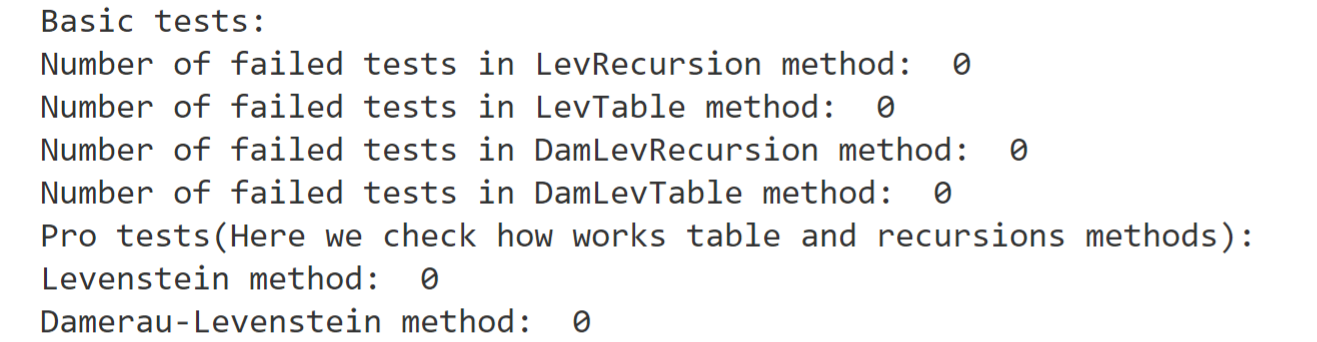
\includegraphics[scale=0.8]{result_tests}
		\centering\caption{Результаты проведенных тестов.}
	\end{figure}
	\subsection{Вывод}
	\hspace*{5mm} В данном разделе была представлена реализация алгоритмов нахождения расстояния Левенштейна, Дамерау-Левенштейна, а также рекурсивные алгоритмы Левенштейна и Дамерау-Левенштейна. Было проведено тестирование направленное на правильность её работы. Все тесты прошли успешно. 
	
\end{flushleft}

\newpage
\section{Исследовательская часть }
\begin{flushleft}
	\hspace*{5mm} В данном разделе будет проведен эксперимент и сравнительный анализ.
	\subsection{Постановка эксперимента}
	В рамках данного проекта были проведены эксперименты, описанные ниже:
	\begin{enumerate}
		\item Сравнение алгоритмов Левенштейна и Дамерау-Левенштейна. Количество символов в слове от 1 до 1000 с шагом 50. Один эксперимент ставился 100 раз;
		\item Сравнение рекурсивного и итеративного алгоритмов Дамерау-Левенштейна. Количество символов в слове от 1 до 6 с шагом 1. Один эксперимент ставился 20 раз;
	\end{enumerate}
	\subsection{Сравнительный анализ на материале экспериментальных данных}
	\hspace*{5mm} Сравнение времени работы алгоритмов Левенштейна и Дамерау-Левенштейна:
	\begin{figure}[h]
		\centering 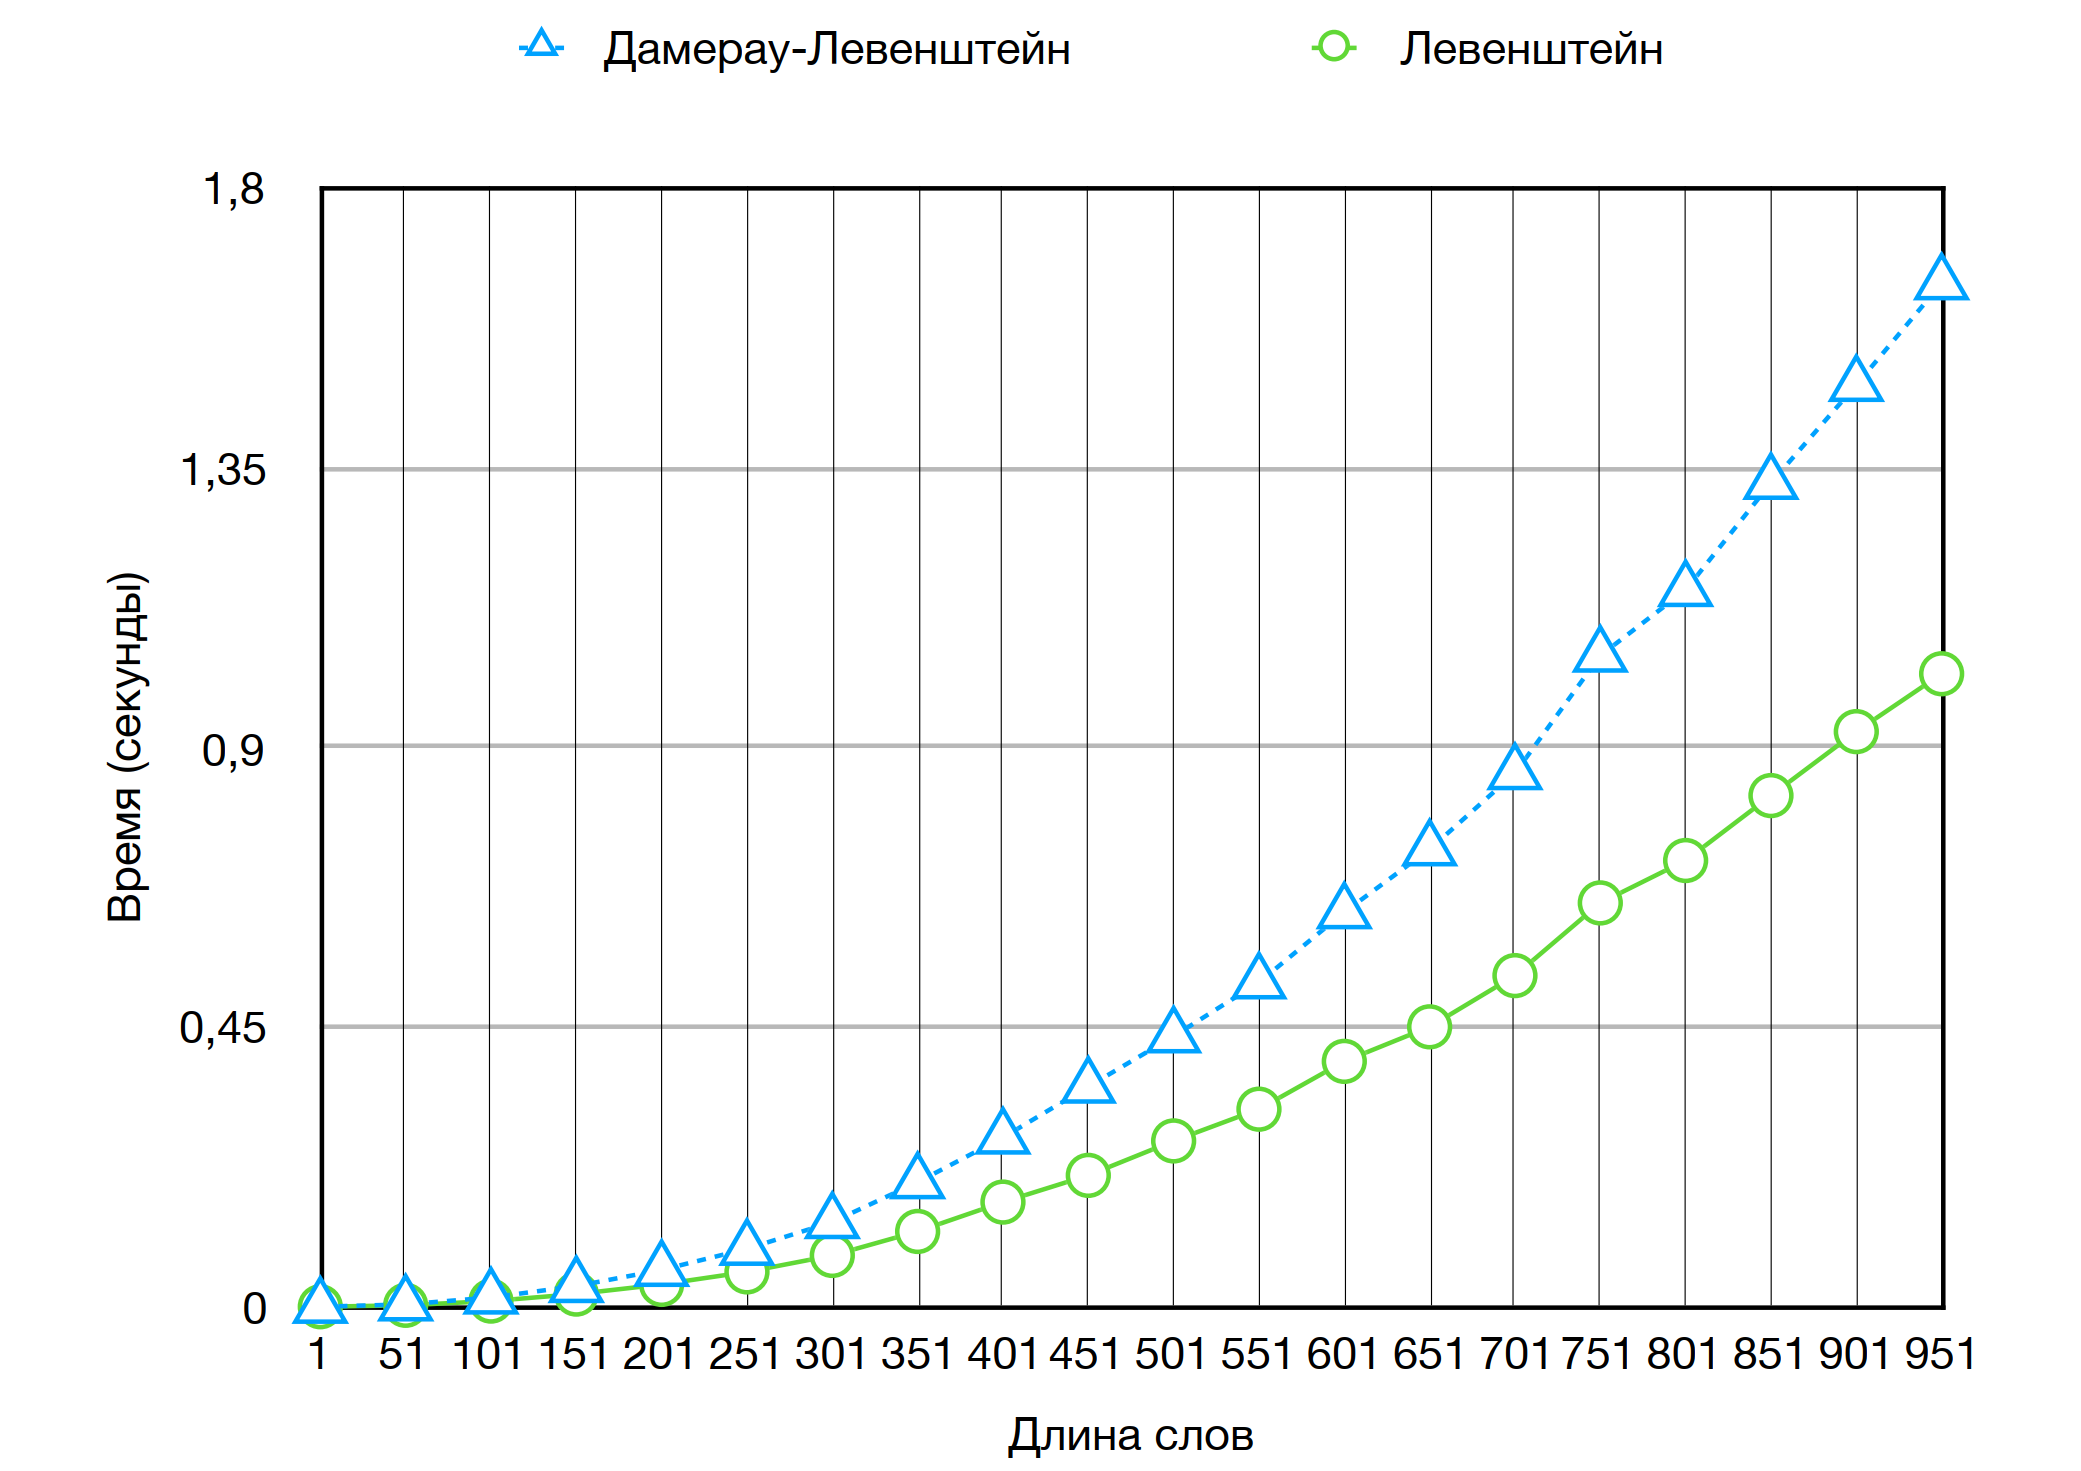
\includegraphics[scale=0.7]{func1}
		\centering\caption{График работы алгоритмов Левенштейна и Дамерау-Левенштейна}
	\end{figure}
	\newpage
	\hspace*{5mm} Можно заметить что алгоритм Дамерау-Левенштейна работает дольше, так как имеет более сложную логику. Также стоит отметить, что оба графика имеет схожий характер. 
	\\ \hspace*{5mm} Сравнение времени работы рекурсивных алгоритмов Левенштейна и Дамерау-Левенштейна:
	\begin{figure}[h]
		\centering 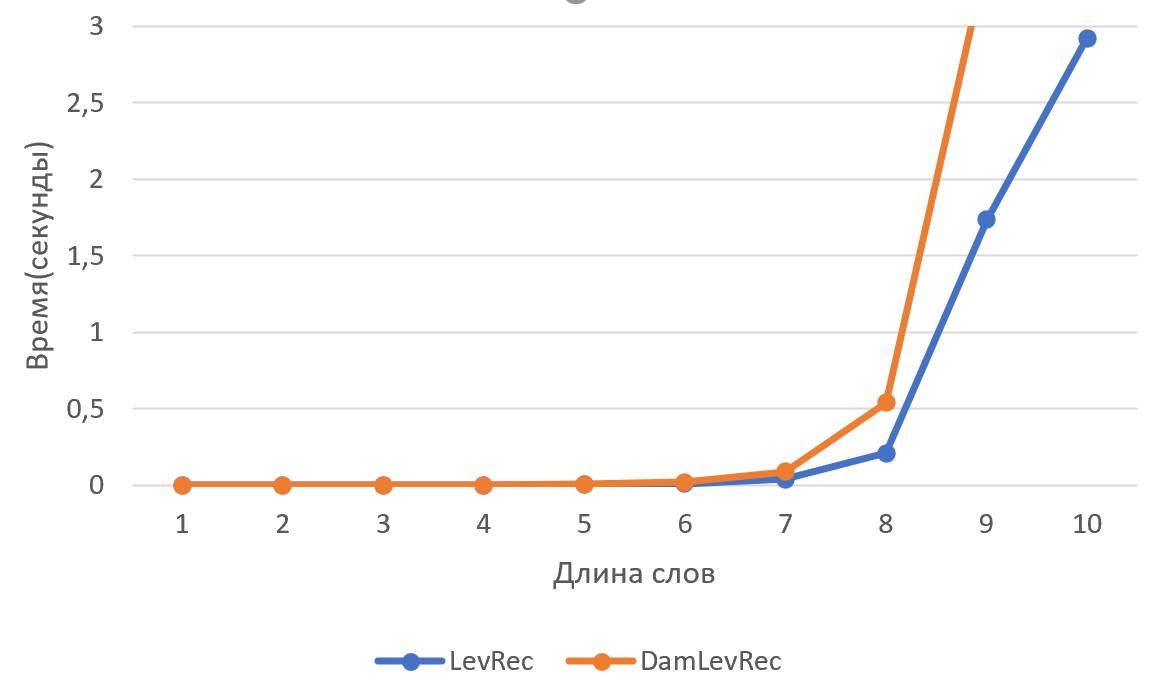
\includegraphics[scale=0.8]{rec}
		\centering\caption{График работы рекурсивных алгоритмов Левенштейна и Дамерау-Левенштейна}
	\end{figure}
	\\ \hspace*{5mm} В приведенном выше графике можно заметить, что оба алгоритмы имеют одинаковый характер, но по скорости рекурсивный алгоритм Левенштейна работает быстрее, чем рекурсивный алгоритм Дамерау-Левенштейна.Замеры рекурсивного алгоритма с итеративным не имеют смысла, так время выполнения рекурсивного алгоритма увеличивается экспоненциально. При одинаковом размере строк рекурсивный алгоритм сильно проигрывает итеративному.
	\subsection{Вывод}
	\hspace*{5mm} В данном разделе был поставлен эксперимент по замеру времени выполнения алгоритма. По итогам замеров алгоритм нахождения расстояния Левенштейна оказался самым быстрым, а самым медленным - рекурсивный алгоритм Дамерау-Левенштейна.
\end{flushleft}

\begin{flushleft}
	\newpage
	\section*{Заключение}
	\hspace*{5mm} В ходе работы были изучены алгоритмы нахождения расстояния Левенштейна и Дамерау-Левенштейна(рекурсивный и итеративный). Выполнено сравнение рекурсивных и итеративных алгоритмов. Изучены зависимости времени выполнения алгоритмов от длин строк. При сравнении времени выполнения алгоритмов, стало понятно, что самый быстрый среди рассматриваемых алгоритмов - алгоритм Левенштейна, а самый медленный рекурсивный алгоритм Дамерау-Левенштейна. Также реализован программный код продукта.  
\end{flushleft}



\end{document}